\documentclass{article}
\usepackage{graphicx} % Required for inserting images
\usepackage{float}
\usepackage[T1]{fontenc}
\usepackage{amsmath}
\usepackage[margin=1in]{geometry}
\usepackage{booktabs}
\usepackage{tabularx}
\usepackage[hidelinks]{hyperref}

\title{Selling 45-DTE puts and closing at 21 DTE on the short-only book}
\author{Experiment report \textperiodcentered{} L/S Gamma Desk, QUANTT}
\date{2026-10-16}

\begin{document}

\maketitle

\textbf{Question:} On the short-only book, does entering near 45 DTE (min 35, max 60) and exiting at 21 DTE raise net P\&L at 1x and 2x spreads, in both halves, without a worse daily tail, compared with the live 30-DTE entry and 7-DTE exit?

\textbf{Method:}

\begin{itemize}

\item \textbf{Pre-registration:} the hypothesis card was committed before any run (commit 1d4144f).

\item \textbf{Data:} the live paper rules (\texttt{configs/\allowbreak{}paper.\allowbreak{}toml}) are replayed on R2 replay snapshots v1 (config\_hash b040760187f0) over the development window 2014-06-02 to 2024-12-31. The hold-out (2025-01-01 to 2026-07-10) was not used.

\item \textbf{Book:} short-only (\texttt{[signal] long\_\allowbreak{}band = -\allowbreak{}inf}): a short put on a Friday expiry, 1 contract, hedged daily at 10:15 ET. The 3-day flat exit, the stop (1x credit), the 50\% profit-take and the 1-day stop cool-off stay as live.

\item \textbf{Variants:}

\begin{itemize}

\item \texttt{dte45} (primary): \texttt{[entry] target\_\allowbreak{}dte = 45,\allowbreak{} min\_\allowbreak{}dte = 35,\allowbreak{} max\_\allowbreak{}dte = 60}; \texttt{[exit] exit\_\allowbreak{}dte = 21}.

\item \texttt{dte45\_\allowbreak{}exit14} (sensitivity, reported only): the same entry, \texttt{exit\_\allowbreak{}dte = 14}.

\end{itemize}

\item \textbf{Comparison:} the registered runs of \texttt{2026-\allowbreak{}10-\allowbreak{}16-\allowbreak{}short-\allowbreak{}only/\allowbreak{}short\_\allowbreak{}only} (the same short-only book with the live 30-DTE entry, 21-45 window, and 7-DTE exit), at the same spread multiple. They were reused, not rerun. Baseline trial 1 (live rules, long and short) is shown in grey for context.

\item \textbf{The full live change:} the VRP signal is measured on the expiry the rule picks. So the variants also compare ATM IV of the expiry near 43 DTE with a GARCH forecast over that horizon, with the same 0.02 short band. The PM approved testing it this way.

\item \textbf{Runs:} every variant ran once at 1x and 2x spreads. Costs are \$0.65 per contract and \$0.005 per share, with a \$1 minimum per order.

\end{itemize}

This report was written by Claude at the PM's request.

\section{Result vs the pass bar}

\texttt{dte45} against \texttt{short\_\allowbreak{}only} at the same spread multiple. Every check had to hold at 1x and 2x. P\&L is net USD on daily equity for 1 contract. ES is the mean of the worst 5\% of daily P\&L.

\begin{center}\small
\begin{tabularx}{\linewidth}{>{\raggedright\arraybackslash}X l l l l >{\raggedright\arraybackslash}X}
\toprule
\textbf{Check} & \textbf{1x value} & \textbf{1x bar} & \textbf{2x value} & \textbf{2x bar} & \textbf{Result} \\
\midrule
Net P\&L, full window & \ensuremath{-}886 & > \ensuremath{-}774 & \ensuremath{-}2,156 & > \ensuremath{-}2,351 & fail 1x, pass 2x \\
Net P\&L, 2014-06 to 2019-12 & \ensuremath{-}559 & > \ensuremath{-}875 & \ensuremath{-}949 & > \ensuremath{-}1,261 & pass \\
Net P\&L, 2020-01 to 2024-12 & \ensuremath{-}327 & > +101 & \ensuremath{-}1,207 & > \ensuremath{-}1,090 & fail \\
abs ES 5\% \ensuremath{\leq} 1.10 \ensuremath{\times} reference & 81.0 & \ensuremath{\leq} 94.1 & 85.4 & \ensuremath{\leq} 101.7 & pass \\
Event floor: round trips (1x) & 95 & \ensuremath{\geq} 30 &  &  & met \\
\bottomrule
\end{tabularx}
\end{center}

\textbf{Verdict: failed.} The 45/\allowbreak{}21 window loses \$112 more than the live window at 1x and \$195 less at 2x. It is better in 2014-2019 at both spreads and worse in 2020-2024 at both. The daily tail is a little lighter. The book still loses money in every variant.

\subsection{Full-window numbers (not part of the bar)}

\begin{center}\small
\begin{tabularx}{\linewidth}{>{\raggedright\arraybackslash}X >{\raggedright\arraybackslash}X l >{\raggedright\arraybackslash}X >{\raggedright\arraybackslash}X l >{\raggedright\arraybackslash}X}
\toprule
\textbf{} & \textbf{short\_only 1x} & \textbf{dte45 1x} & \textbf{dte45\_exit14 1x} & \textbf{short\_only 2x} & \textbf{dte45 2x} & \textbf{dte45\_exit14 2x} \\
\midrule
Net P\&L & \ensuremath{-}774 & \ensuremath{-}886 & \ensuremath{-}575 & \ensuremath{-}2,351 & \ensuremath{-}2,156 & \ensuremath{-}1,756 \\
Round-trip P\&L before commissions & +318 & +817 & +1,221 & \ensuremath{-}1,240 & \ensuremath{-}433 & +59 \\
Sharpe on \$250k & \ensuremath{-}0.15 & \ensuremath{-}0.19 & \ensuremath{-}0.12 & \ensuremath{-}0.42 & \ensuremath{-}0.44 & \ensuremath{-}0.36 \\
Max drawdown & 2,220 & 1,957 & 1,951 & 3,222 & 2,882 & 2,494 \\
ES 5\% (daily) & \ensuremath{-}85.5 & \ensuremath{-}81.0 & \ensuremath{-}79.4 & \ensuremath{-}92.4 & \ensuremath{-}85.4 & \ensuremath{-}83.6 \\
Round trips & 100 & 95 & 91 & 100 & 95 & 91 \\
Commissions (options /\allowbreak{} hedges) & 200 /\allowbreak{} 770 & 190 /\allowbreak{} 714 & 182 /\allowbreak{} 716 & 200 /\allowbreak{} 770 & 190 /\allowbreak{} 714 & 182 /\allowbreak{} 716 \\
\bottomrule
\end{tabularx}
\end{center}

\section{Charts}

\begin{figure}[H]\centering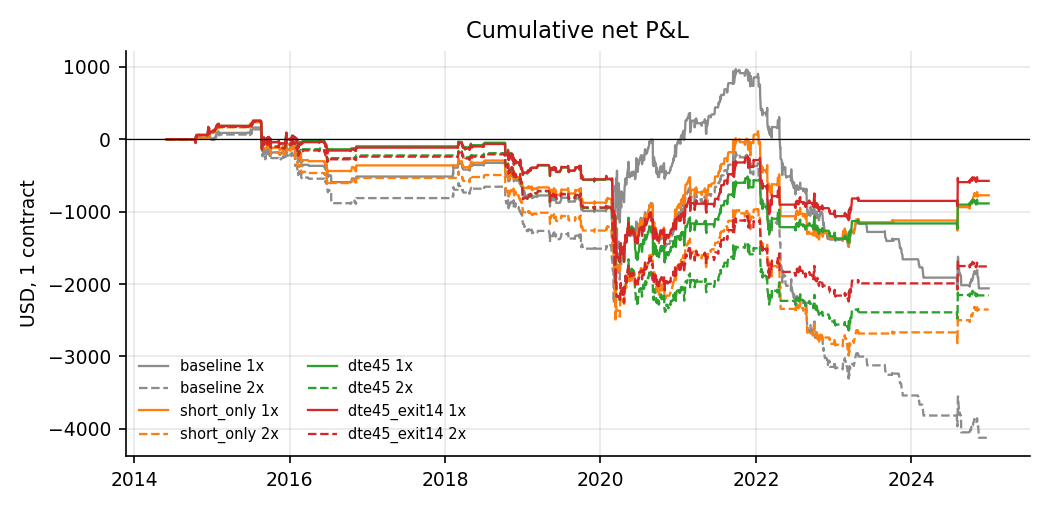
\includegraphics[width=0.92\linewidth]{figures/cum_pnl.png}\caption{Cumulative net P\&L, 1x solid and 2x dashed; baseline (live rules) grey}\end{figure}

\texttt{dte45} runs slightly ahead of the reference from 2016 to 2019. It falls behind in 2020 and catches up in the 2022 sell-off, where it loses much less. It then drifts behind again in 2023-2024. At 1x it ends \$112 behind; at 2x it ends \$195 ahead, because it pays less in spreads.

\begin{figure}[H]\centering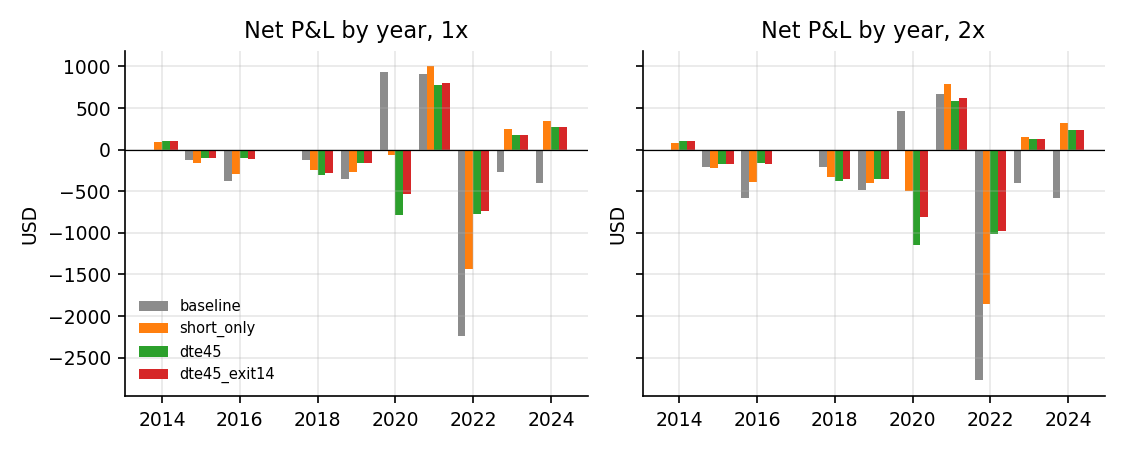
\includegraphics[width=0.92\linewidth]{figures/yearly.png}\caption{Net P\&L by year}\end{figure}

At 1x, \texttt{dte45} is ahead of the reference in 2014-2016, 2019 and 2022 (\ensuremath{-}\$772 against \ensuremath{-}\$1,433). It is behind in 2018, 2020, 2021, 2023 and 2024. 2020 alone accounts for \ensuremath{-}\$720 (\ensuremath{-}\$780 against \ensuremath{-}\$60), mostly in February-March and June, when the two books entered on different days. So this is path dependence on a handful of trades. 2017 has no trades in any variant.

\begin{figure}[H]\centering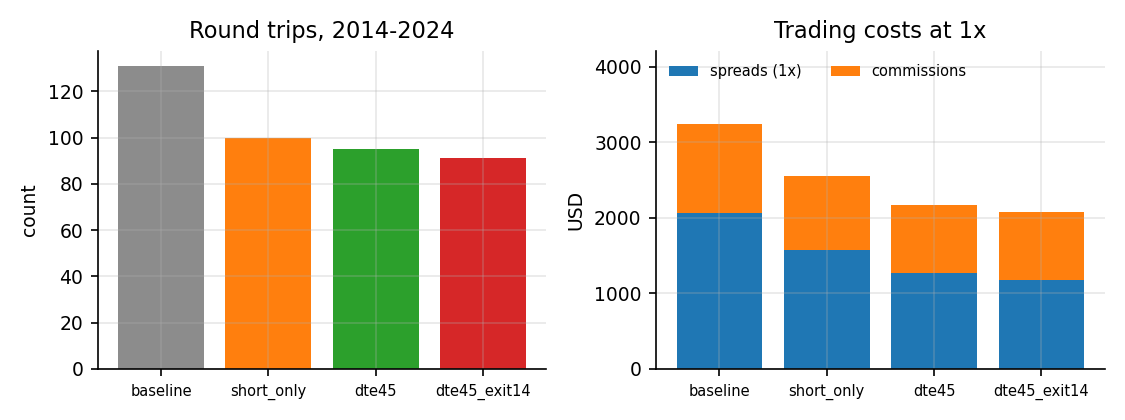
\includegraphics[width=0.92\linewidth]{figures/costs.png}\caption{Round trips and trading costs at 1x}\end{figure}

This chart shows the cost side. The 45-DTE window trades a little less (95 round trips against 100) and costs less to trade. At 1x, spreads (1x minus 2x equity P\&L) fall from \$1,578 to \$1,270, and commissions from \$970 to \$904: \$373 less in total. At 2x the spread saving doubles, so the cost advantage is about \$680.

\begin{figure}[H]\centering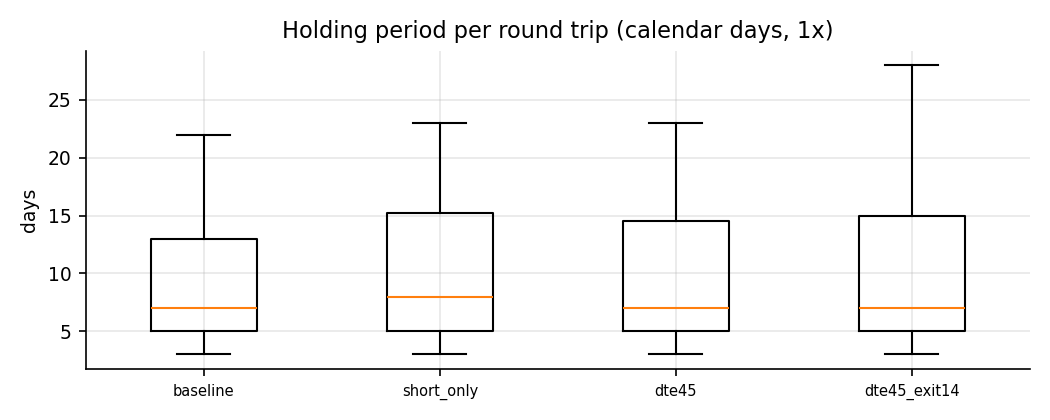
\includegraphics[width=0.92\linewidth]{figures/holding.png}\caption{Holding period per round trip}\end{figure}

Holding periods barely change: a median of 7 days for \texttt{dte45} against 8 for the reference, and a mean of 10.2 against 10.7. The 3-day flat exit still closes most trades (82 of 95) long before either time exit.

\begin{figure}[H]\centering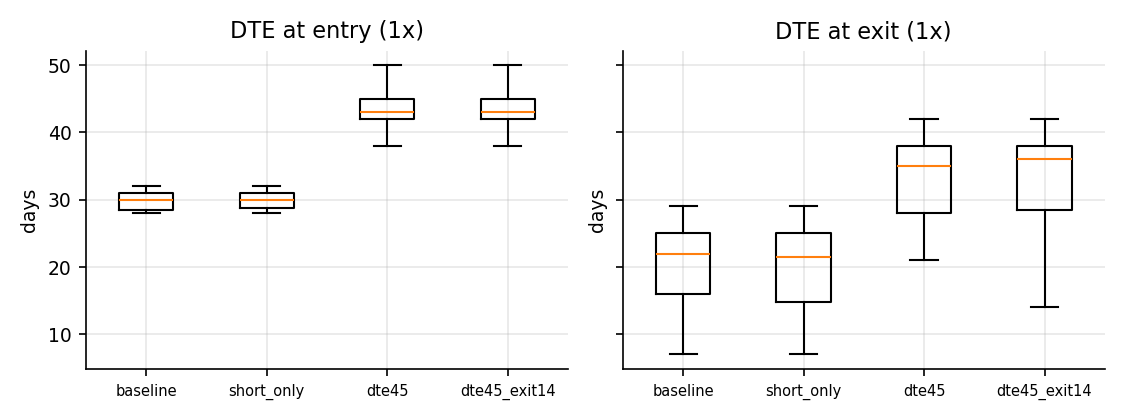
\includegraphics[width=0.92\linewidth]{figures/dte.png}\caption{DTE at entry and at exit, 1x}\end{figure}

Entries move from a median 30 DTE to 43 DTE (5th-95th percentile 38-50). Most trades close on the flat exit after about a week, so the median exit moves from 22 DTE to 35 DTE. The 45-DTE book almost never holds a contract inside 21 DTE (2 of 95 trades closed below 21). Half of the reference's trades (50 of 100) closed at 21 DTE or less.

\begin{figure}[H]\centering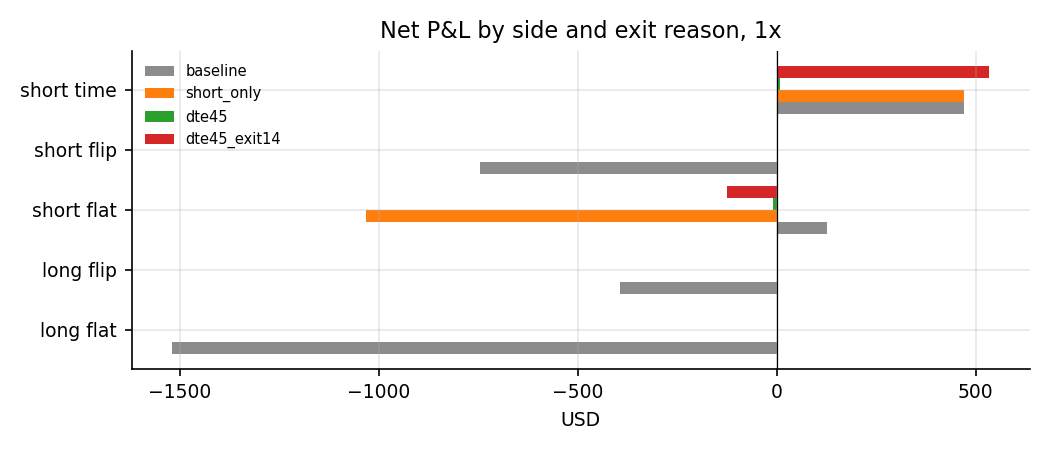
\includegraphics[width=0.92\linewidth]{figures/by_reason.png}\caption{Net P\&L by side and exit reason, 1x}\end{figure}

Round-trip net P\&L (subject to the marking issue in the analysis) is about zero for \texttt{dte45} in both groups: \ensuremath{-}\$9 from 82 flat exits and +\$8 from 13 time exits at 21 DTE. The reference's 13 time exits at 7 DTE made +\$470, and its flat exits lost \$1,032. No stop or profit-take fired in any of these variants.

\begin{figure}[H]\centering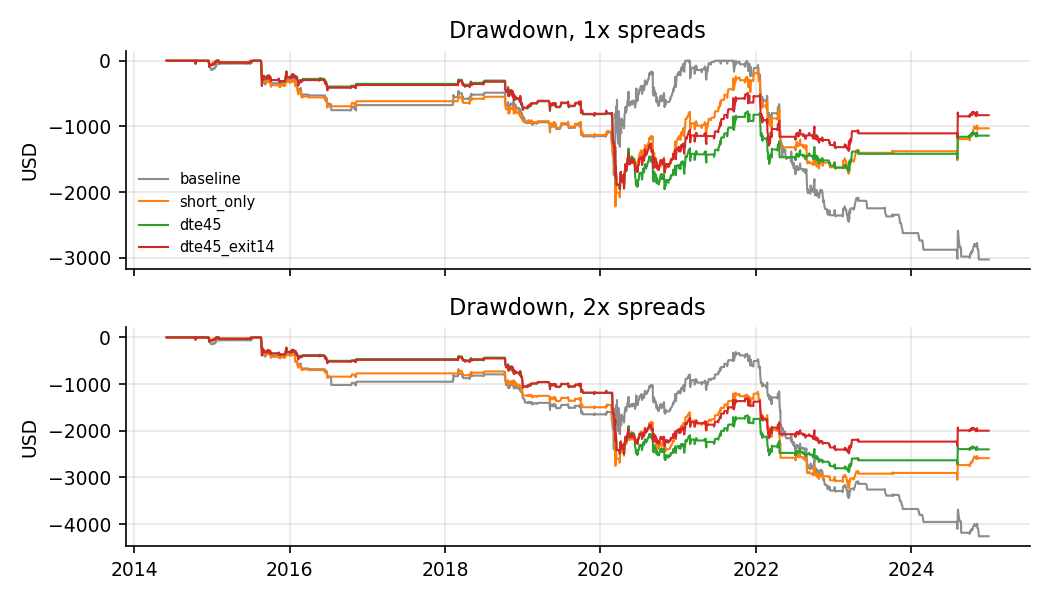
\includegraphics[width=0.92\linewidth]{figures/drawdown.png}\caption{Drawdown at 1x and 2x spreads}\end{figure}

The maximum drawdown is smaller for \texttt{dte45} at both spreads: \$1,957 against \$2,220 at 1x, and \$2,882 against \$3,222 at 2x. The worst day in every short-only variant is 2020-03-12, where \texttt{dte45} lost \$406 against \$703 for the reference.

\begin{figure}[H]\centering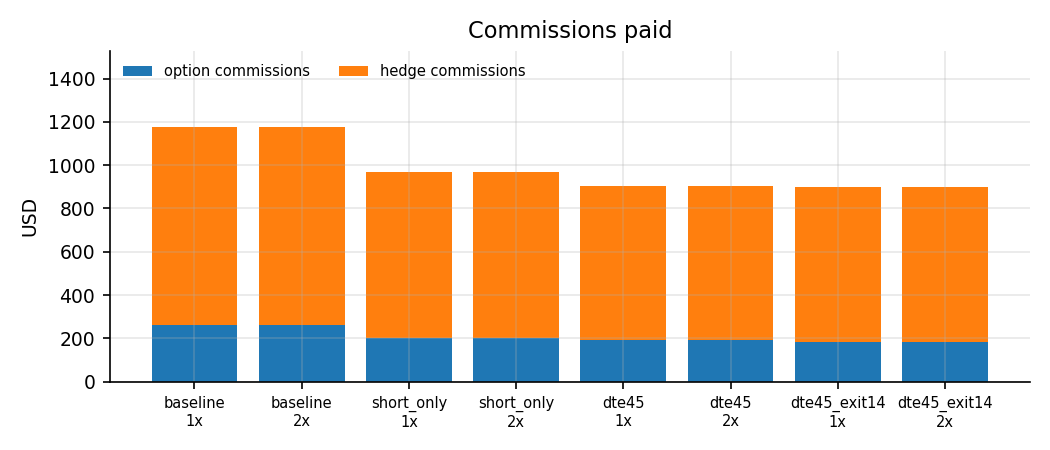
\includegraphics[width=0.92\linewidth]{figures/fees.png}\caption{Commissions paid}\end{figure}

Hedge commissions are about 80\% of commissions in every short-only variant. \texttt{dte45} places 714 hedge orders against 770 and trades 11\% fewer hedge shares.

\section{Analysis}

The 45/\allowbreak{}21 window changes three things at once: a longer-dated contract, a VRP signal measured on that contract, and a time exit that, with the flat exit, keeps the book out of the last three weeks. The signal barely moves. It is short on 430 of 2,576 signal days against 466, and the two agree on 96\% of days. 59 of the 95 \texttt{dte45} round trips start on the same day as a reference trade. So most of the difference is in what each trade holds, not when it trades.

\subsection{P\&L bridge}

At 1x (\texttt{dte45} minus \texttt{short\_\allowbreak{}only}): round-trip P\&L before commissions +\$500 (+\$817 against +\$318), commissions +\$66, and the unattributed unwind residual \ensuremath{-}\$678 (\ensuremath{-}\$799 against \ensuremath{-}\$122), giving \ensuremath{-}\$112. At 2x: +\$807, +\$66 and \ensuremath{-}\$678, giving +\$195. The residual is equity P\&L minus round-trip P\&L net of all commissions.

\begin{itemize}

\item \textbf{Cheaper to trade, by about \$370 at 1x.} Spreads fall \$307 and commissions \$66. The option spread per round trip falls from about \$15.1 to \$12.8. For an option of the same price, the spread model's 31-60 DTE fit is cheaper than its shorter-dated fits. The 30-DTE short closes at 7-29 DTE, while the 45-DTE short mostly closes at 28-38 DTE. Fewer days in the market (969 against 1,067) and lower gamma also mean 11\% fewer hedge shares and 56 fewer hedge orders. These savings are mechanical, and the spread part doubles at 2x.

\item \textbf{Less P\&L before costs, by about \$485.} Adding the 1x spreads and commissions back to equity P\&L gives +\$1,774 for the reference and +\$1,288 for \texttt{dte45}. Closing at about 35 DTE gives up the faster decay that a 30-DTE short collects, and the reference's 13 trades held to 7 DTE were its best group. At 1x the lost P\&L is larger than the cost saving; at 2x it is smaller.

\item \textbf{The round-trip gross overstates the gain.} Each round trip marks its option close at the fill-window price but its hedge shares at the decision spot. The order that flattens the hedge fills 15-30 minutes after the decision data. So each trip's P\&L carries the option's unhedged move over that gap, and equity corrects it. Summed over all closes, that gap is \ensuremath{-}\$765 for \texttt{dte45} and \ensuremath{-}\$71 for the reference. It is noise: the spot move between decision and fill has a standard deviation of about \$1.2-1.3 per close in both runs. The per-trip residual has a standard deviation of about \$80, so the sum over 95 trips has a standard deviation of roughly \$750-800. The pass bar uses equity P\&L, which is the true number. But the +\$500 gross gain should not be read as a decay gain.

\end{itemize}

\subsection{Halves and the sensitivity variant}

The second half fails mainly because of 2020 (\ensuremath{-}\$720 at 1x), and 2022 (+\$661) almost offsets it. 2021, 2023 and 2024 are each \$67-229 behind. Without 2020 the second half would have been ahead at both spreads, but 2020 is in the window and the bar is per half. The first-half gain (+\$316 at 1x) comes mostly from 2016 (+\$192) and 2019 (+\$111).

\texttt{dte45\_\allowbreak{}exit14} holds the longer trades to 14 DTE (8 time exits, +\$534 net). It beats the reference at 2x over the full window and in both halves, and at 1x over the full window (\ensuremath{-}\$575 against \ensuremath{-}\$774). It still fails the 2020-2024 half at 1x (\ensuremath{-}\$22 against +\$101). It was reported only, and its edge is also within the size of the unwind noise.

\section{Verdict}

\textbf{Failed} on the pre-registered bar: the 1x full window and the 2020-2024 half at both spreads fail. Keep the live 30-DTE entry and 7-DTE exit.

The honest reading: on this book the 45/\allowbreak{}21 window is roughly neutral. It trades more cheaply and with a lighter tail, and it gives up about as much P\&L as it saves in costs. The 2x gain (+\$195) and the 1x loss (\ensuremath{-}\$112) are both smaller than the unwind noise. A follow-up would need its own card and would be in-sample, for example 45-DTE entries held to 14 DTE on the short-only book with the 10-share hedge band.

\section{Caveats}

\begin{itemize}

\item \textbf{In-sample:} the idea comes from the 2026-10-16 desk discussion of the baseline on this same window.

\item \textbf{One contract:} the \$1 minimum per order is large relative to size, and hedge orders are most of the commissions.

\item \textbf{Spread model:} fitted on about two weeks of calm 2026 live quotes, with separate fits by DTE. Part of the cost saving comes from those fits. The 2x run is the stress test.

\item \textbf{Data gaps:} R2 has no month-end weekdays, so 89 scheduled times (3.3\%) are skipped in every variant.

\item \textbf{Edge of the chain:} the replay chain lists expiries up to 60 DTE, and expiries with too few trades for a smile fit are dropped. The rule picked a median 43 DTE, not 45 (38-50 DTE for 90\% of entries).

\item \textbf{Embargo:} entries stop \texttt{max\_\allowbreak{}dte} days before the hold-out, so the variants make no entries after 2024-11-01 (reference: 2024-11-16). Both books were holding a short through their last short-signal days of 2024 (the last on 2024-11-05) and had no short signal after their final closes (2024-11-08 and 2024-11-07), so the earlier embargo blocked no entry.

\item \textbf{Few events per half:} 38 round trips in 2014-2019 and 57 in 2020-2024 for \texttt{dte45}. The yearly differences rest on a handful of trades each.

\item \textbf{Unwind noise:} the hedge-flattening orders fill on a spot 15-30 minutes after the decision data. Over a run, that noise is larger than the margins in this test.

\end{itemize}

\section{Trials}

4 trials for this experiment (2 variants at 1x and 2x, one run of \texttt{experiment.\allowbreak{}py}), plus the baseline's 2. The reference was reused from \texttt{2026-\allowbreak{}10-\allowbreak{}16-\allowbreak{}short-\allowbreak{}only} (2 trials, not rerun). The pass bar was not changed.

\end{document}
